\chapter[TIC en la Educación]{Tecnologías de la Información y Comunicación en
    la Educación}
\label{chap:tics}

% TODO: Unificar los ejemplos para que sean más simples, para ver lo de los
% juegos serios y el construccionismo

Las \Gls{tic} son el conjunto de herramientas tecnológicas y recursos utilizados
para comunicar, crear, diseminar, almacenar y manejar la
información\cite{unesco:ict}. Estas tecnologías abarcan computadores personales,
Internet, radio, televisión y telefonía\cite{tinio:ict}.

La utilización actual de las \Gls{tic} en la educación no es un fenómeno
asilado, responde a una evolución constante de la tecnología y metodología
utilizada\cite{egenfeldt2007third}. Las expectativas iniciales acerca del
impacto de las \Gls{tic} en la educación han sido ampliamente superiores a los
resultados obtenidos\cite{unesco:ict}. Con el advenimiento de las computadoras
se redujo la diferencia entre las expectativas y lo obtenido, en mayor medida
por la utilización de las \Gls{tic} en conjunto con tecnologías como Internet,
así, los efectos positivos en la educación han aumentando
gradualmente\cite{unesco:ict}.

Desde sus inicios, varias corrientes pedagógicas emplean a las \gls{tic} en
mayor o menor medida, desde su utilización como una herramienta para suplantar a
libros impresos, diapositivas, etc\cite{nanjappa2003constructing}; hasta su
utilización como una herramienta de aprendizaje de pensamiento de alto
nivel\cite{egenfeldt2007third,white:ict,nanjappa2003constructing}.

Las corrientes pedagógicas que utilizan a las \Gls{tic} de manera activa son el
instruccionismo o educación tradicional, el conductismo, el constructivismo, y
el construccionismo. Esto no implica que las \Gls{tic} no sean utilizadas por
otras pedagogías, es más, existen otras corrientes que emplean a las \Gls{tic}
de diversas maneras como el
cognoscitivismo\cite{egenfeldt2007third,martin2008modelo} y el
conectivismo\cite{white:ict}.

Cada corriente pedagógica utiliza las \Gls{tic} de manera diferente, si bien
comparten características, no deben ser consideradas como una sucesión de
pedagogías que desembocan en una pedagogía utilizada actualmente.

En este capítulo se describen las corrientes pedagógicas que utilizan las
\gls{tic} de manera activa, incluyendo sus características, ventajas y
desventajas. Finalmente se describen las ventajas y desafíos que presenta la
utilización de las \Gls{tic} en la educación.

\section[Breve reseña histórica]{Breve reseña histórica de la utilización de las
    \gls{tic} en la educación}

El análisis de la historia de las \Gls{tic} en educación es
indispensable\cite{mcdougall2006theory}. Existe una corriente que tiende a
desestimar las experiencias pasadas, cuyo principal fundamento es la velocidad
con la que la tecnología evoluciona, es importante el estudio de la evolución de
la misma pues los errores pedagógicos cometidos, aunque puedan parecer evidentes
hoy en día, condujeron a nuevos modelos y conclusiones que son la base de la
utilización de las \Gls{tic} actualmente\cite{mcdougall2006theory}. Así, el uso
de las \Gls{tic} en la educación no ha sido constante durante su historia, sino
más bien, ha evolucionado de ser un medio más de traspaso de información, hasta
hoy en día, donde permite construir conocimiento\cite{tinio:ict}.

La historia de las \Gls{tic} en educación comienza en la \enquote{Open
    University of United Kingdom} que en $1969$ se establece como la primera
institución educativa dedicada a la enseñanza a distancia utilizando las, para
aquel entonces, nuevas tecnologías\cite{tinio:ict}.

Para entender la historia de las \Gls{tic} en la educación, se presenta la
figura~\ref{fig:history_tics}, en la cual se observa la evolución que sufrió la
utilización de las \Gls{tic} como herramienta educativa. 

\begin{figure}[h]
\centering
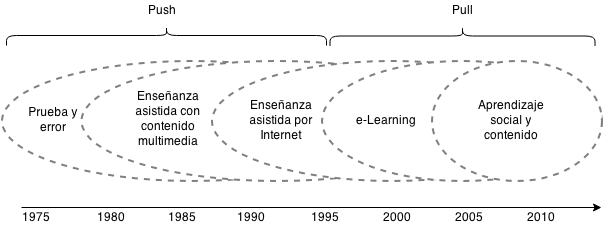
\includegraphics[scale=0.75]{tics/images/tics_history.png}
\caption{Utilización de las \Gls{tic} en la educación desde el año $1975$. Las
    fechas utilizadas son relacionadas a la evolución en los Estados Unidos de
    Norte America.}
\label{fig:history_tics}
\end{figure}



%Se observa que se
%parte la historia en cinco corrientes definidas, y a la vez, estas corrientes se
%agrupan según el mecanismo de traspaso de información, las tres primeras
%corrientes se denominan \textit{push} y las siguientes dos se denominan
%\textit{pull}. 

Se observan dos metodologías de traspaso de la información, \textit{push}, y
\textit{pull}. En el modelo \textit{push} los estudiantes obtienen información
sin una participación activa en la creación de esa información\cite{white:ict}.
La corrientes pedagógicas que marcan tendencia en este modelo son el
instruccionismo y el conductismo\cite{white:ict,leinonen:ict}. Las fases que se
observan en la figura~\ref{fig:history_tics} durante el periodo \textit{push},
son la utilización de ejercicios de prueba y error sistemáticos, y la
distribución de contenido educativo primeramente a través de discos ópticos, y
luego a través de Internet\cite{leinonen:ict}.

La evolución de la tecnología permite mejorar los mecanismos de comunicación,
creando redes interactivas donde se comparte la información, así se inicia el
modelo \textit{pull}, en él, los alumnos son creadores activos de
conocimiento\cite{white:ict,leinonen:ict}. Se intensifica la creación de
herramientas basadas en el constructivismo y el construccionismo. Ejemplos de
las tecnologías en este período son el \textit{e-Learning}, y plataformas de
interacción social como wikis, blogs, y otros\cite{leinonen:ict}.

En la figura~\ref{fig:history_tics} se observa el solapamiento entre los
diversos mecanismos utilizados. Se muestra el inicio de la utilización de una
herramienta, pero no su fin, actualmente se siguen utilizando todas las
tecnologías y modelos\cite{leinonen:ict}.

Aunque la figura~\ref{fig:history_tics} muestre un progreso lineal de las
corrientes, este progreso no es igual en todo el mundo, y el grado de impacto de
las \Gls{tic} varia entre países, lo que se conoce como \enquote{brecha
    tecnológica}.


\section{Teorías del aprendizaje: Modelo Push}


La primera manifestación de las \gls{tic} en la educación se da como un
sustituto a los medios tradicionales. Los materiales didácticos son
responsabilidad de los profesores, imprentas y
academias\cite{leinonen:ict,white:ict}.

El modelo \textit{push} favorece a las corrientes pedagógicas instruccionismo y
conductismo. El instruccionismo utiliza a las \gls{tic} para resolver problemas
de distancia y de costo\cite{igi:instructionism,johnson2005instructionism},
mientras que el conductismo utiliza a las \gls{tic} como un medio para proveer
refuerzos positivos\cite{weegar2012comparison}.

\subsection{Instruccionismo}

La educación tradicional o instruccionismo se basa en la transferencia de
conocimiento del profesor al alumno, se enfoca más en el profesor, en la
capacidad del mismo, y en el producto final como resultado de un proceso no
interactivo y bien
documentado\cite{igi:instructionism,johnson2005instructionism}. Los mecanismos
tradicionales para probar la efectividad de este tipo de enseñanza son los
exámenes escritos.

El instruccionismo es conocido además como enseñanza sistemática, enseñanza
explícita, enseñanza directa, y enseñanza
activa\cite{johnson2005instructionism}. Siempre se enfatiza en el
profesor\cite{johnson2005instructionism}.

Epistemológicamente se puede observar al instruccionismo como objetivo, pues
considera que el conocimiento es independiente del entorno, se asume que el
mismo es isomorfo, si el profesor puede enseñar, el alumno puede
aprender\cite{johnson2005instructionism}.

En el instruccionismo, la utilización de las \Gls{tic} se centra principalmente
en mecanismos para proveer contenido, se utilizan plataformas que
permiten a los profesores distribuir contenido y otras actividades relacionadas.

\subsubsection{Ejemplos}

Las aplicaciones de las \gls{tic} en el instruccionismo son:

\begin{itemize}

\item \textbf{E-Learning}: El \emph{E-Learning} se define como la educación y
    capacitación a través de medios digitales, incluye todo tipo de medio capaz
    de distribuir información, puede ser en tiempo real como salas de
    conversaciones y videoconferencias o puede ser diferido, como por ejemplo
    foros y enciclopedias\cite{punie:ict}.

    Una de las desventajas del \emph{e-Learning} es que se distribuye contenido
    masivamente a los alumnos, y luego, de manera discreta se permite a los
    mismos colaborar, dejando siempre en claro que primero se debe asimilar toda
    la información posible y luego relacionarse con los
    demás\cite{leinonen:ict}, es decir, los alumnos no forman parte de la
    creación del conocimiento.

    \begin{figure}[h] 
    \centering 
    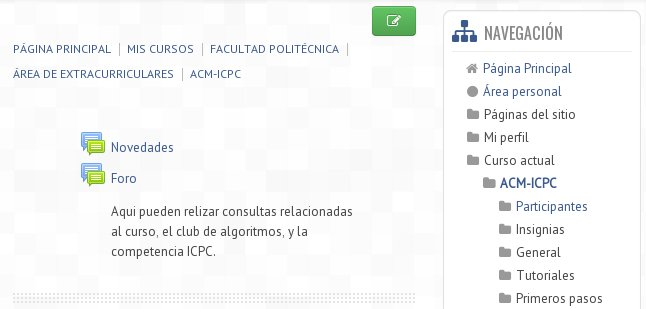
\includegraphics[scale=0.5]{tics/images/moodle.jpg}
    \caption{Moodle, plataforma de e Learning}\label{fig:moodle}
    \end{figure}

    La plataforma \emph{Moodle} (ver figura~\ref{fig:moodle}) cuya primera
    versión salió en el $2002$, es una de las principales herramientas del
    \emph{e-Learning} hoy en día, permite la creación de cursos específicos por
    materia y sitios especializados por instituciones
    académicas\cite{perkins2006using}. 

\item \textbf{Sustituto de medios tradicionales}: la utilización de las
    \gls{tic} desde sus inicios es como sustituto de los medios físicos, como
    libros y diapositivas por sus versiones digitales\cite{tinio:ict}.

\item \textbf{Clases a distancia}: las clases por videoconferencias y clases
    grabadas en video son herramientas utilizadas en reemplazo de las clases
    tradicionales. Permiten eliminar las distancias de tiempo y
    espacio\cite{tinio:ict}.

\end{itemize}

\subsection{Conductismo}

El conductismo es una corriente de la psicología, creada por \textit{Jhon
    Watson}, y posteriormente perfeccionada por \textit{Pavlov},
\textit{Skinner}, y \textit{Thorndik}. El conductismo defiende la idea de que
todas las acciones que realizan los seres vivos son consecuencia de un
estímulo\cite{weegar2012comparison}.

La primera utilización del conductismo con las \Gls{tic} es presentada por
\textit{Skinner}, en $1958$\cite{weegar2012comparison}, donde se describe una
máquina que contiene botones y una pantalla donde se presenta una pregunta, para
responder, el usuario dispone de varias opciones, cada opción esta relacionada
con un botón, si el aprendiz no presiona el botón correcto, debe seguir
intentando hasta responder correctamente y así
poder avanzar\cite{weegar2012comparison}, este es el inicio de lo que se conoce como
\enquote{Prueba y Error}.

Una característica del conductismo, es la ley de \textit{Thorndike}, la cual
indica que una acción, cuya consecuencia es un estímulo favorable, es más
probable que sea repetida\cite{weegar2012comparison}.

%A finales de la década de $1970$ e inicios de la década de $1980$,  la
%complejidad técnica de las computadoras limitaba la cantidad de herramientas
%disponibles, los programas eran desarrollados por profesores, y su objetivo era
%que los alumnos puedan poner en práctica lo aprendido en el aula. 

%\textbf{Aprendizaje como anexo:} el principal objetivo del desarrollo de un
%\emph{edutainment} es el de entretener, los objetivos pedagógicos son agregados
%al final. Adicionalmente, este aprendizaje se provee a través de largos textos
%que normalmente son omitidos.

\subsubsection{Ejemplos}
\label{sec:edutainment}

Entre los ejemplos de aplicación del conductismo en las \gls{tic} se encuentran:

\begin{itemize}

\item \textbf{Ejercicios de prueba y error}: son ejercicios en los cuales se
    presenta una pregunta y una lista de respuestas al alumno, y este debe
    responder correctamente. Si el alumno no responde correctamente, se repite
    la pregunta\cite{weegar2012comparison}.

\item \textbf{Edutainment}: son juegos sencillos que transmiten información
    simple al usuario, su estructura se basa en un objetivo claro que está
    separado de la experiencia educativa\cite{egenfeldt2007third}. El
    \emph{edutainment} pretende agregar entretenimiento a la educación, se ve al
    alumno como un receptor pasivo de información que debe asimilarla, y para
    aumentar la implicación de los alumnos, el entretenimiento es
    agregado\cite{resnick:2004}. Los \emph{edutainment} son el primer intento de
    unir el entretenimiento y la educación dentro de las
    \gls{tic}\cite{leinonen:ict}.

    Entre ejemplos de los \emph{edutainment}, podemos encontrar a:

    \begin{itemize}

    \item \textbf{Math Blaster}: (ver figura~\ref{fig:math_blaster}) es un
        \emph{edutainment} donde el alumno debe responder repetitivamente
        preguntas aritméticas para obtener municiones, luego con esas municiones
        debe completar diferentes misiones en una nave\cite{bruckman1999can}.
        Como todas las preguntas se responden mediante un mecanismo de selección
        múltiple, y no existe penalización por respuestas incorrectas, los
        alumnos no reflexionan sobre las respuestas elegidas, seleccionan una
        opción aleatoria y si no es la correcta, prueban otra, tras una cantidad
        finita de intentos, siempre se obtiene la recompensa deseada.

        \begin{figure}[ht!] 
        \centering 
        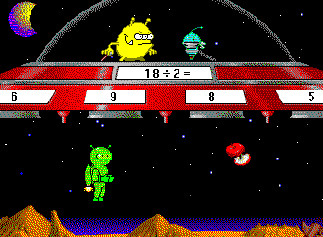
\includegraphics[scale=0.5]{tics/images/math_blaster.jpg}
        \caption{Math Blaster, \emph{edutainment} del año 1987}\label{fig:math_blaster} 
        \end{figure}

    \item \textbf{Donde en el mundo esta Carmen Sandiego} (ver
        figura~\ref{fig:carmen}) el objetivo del juego es detener a una serie de
        criminales mediante indicios que son proveídos en forma de texto. Este
        exitoso juego demuestra las falencias del \textit{Edutainment}, siendo
        visualmente muy atractivo, y con contenido multimedia acorde a su
        tiempo, no era más que \enquote{Prueba y Error}, cada nivel del juego
        podía ser completado sin leer la información
        proveída\cite{charsky:2010}.

        \begin{figure}[ht!] 
        \centering 
        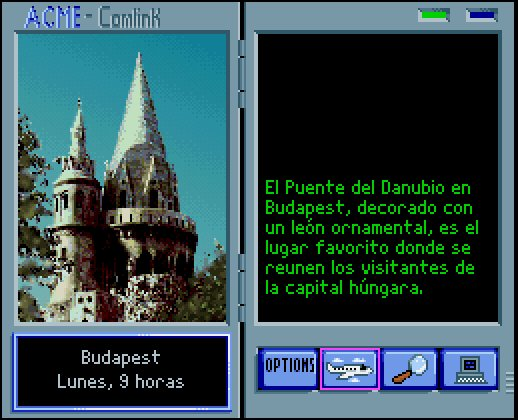
\includegraphics[scale=0.5]{tics/images/carmen.jpg}
        \caption{Donde en el mundo esta Carmen Sandiego}\label{fig:carmen}
        \end{figure}

    \end{itemize}

    Las aplicaciones se limitaban a matemáticas, lenguaje y geografía, donde se
    podía evaluar inmediatamente los resultados proveídos por los alumnos, pues,
    normalmente era un enunciado y una lista posible de opciones del tipo
    \enquote{Prueba y Error}\cite{leinonen:ict}. 

\end{itemize}

\subsection{Ventajas y desventajas del modelo Push}

Las ventajas del modelo \textit{push} son:

\begin{itemize}

\item Permite controlar el entorno del aprendizaje utilizando un enfoque
    científico. Se controla el entorno de los alumnos, los estímulos que recibe
    y las consecuencias de estos estímulos. Se ignora a los pensamientos y
    experiencias previas de las personas\cite{weegar2012comparison}.

\item Permite educar a personas con desafíos de aprendizaje y
    comportamiento\cite{johnson2005instructionism}.

\item Permite la enseñanza de pensamiento de bajo nivel\footnote{El pensamiento
        de bajo nivel está relacionado con las prácticas educacionales que
        incluyen la capacidad de memorizar y procesar, al contrario, el
        pensamiento de alto nivel incluye la capacidad de crear y
        evaluar\cite{edwards2000higher}}. Son excelentes para enseñar matemática
    básica, geografía y lenguaje\cite{charsky:2010}.

\end{itemize}

Las desventajas que presentan las corrientes del tipo \textit{push} son:

\begin{itemize}

\item No tienen en cuenta la experiencia previa de los alumnos ni el factor
    social. Los medios utilizados para la educación se centran en el profesor y
    en la manera de dar la clase\cite{siemens2008learning,sawyer2005cambridge}.

    El comportamiento humano no puede ser reducido, no solo responde a los
    estímulos y al entorno, sino, además responde a la experiencia
    previa\cite{weegar2012comparison}.

\item No se enfoca en los alumnos, no todos los alumnos aprenden al mismo
    nivel\cite{johnson2005instructionism}.

\item Desde el aspecto pedagógico, los alumnos tienen problemas para comprender
    ideas diferentes a las encontradas en clase\cite{sawyer2005cambridge}.

\item Los alumnos tienden a memorizar contenido sin entender el contexto en el
    cual fue creado el conocimiento\cite{sawyer2005cambridge}. 
    
\item Los alumnos tratan a los hechos y procedimientos como conocimiento
    estático, que no puede ser transformado, y que siempre es
    verdad\cite{sawyer2005cambridge}.

\item Se centra en motivaciones externas, y deja de lado la motivación interna.
    Las motivaciones externas son las recompensas que reciben los alumnos al
    llevar a cabo un ejercicio de manera correcta. La motivación interna es de
    gran importancia\cite{weegar2012comparison}.
    
\item Prueba y error, las aplicaciones creadas utilizando estas corrientes
    permiten al alumno intentar varias veces sin ser penalizados, además de que
    los alumnos no están motivados, provocan que el alumno pruebe las opciones
    sin el proceso de reflexión necesario para aprender. Es decir, se enseñaba a
    probar opciones sin sentido antes que entender y analizar la
    experiencia\cite{charsky:2010,egenfeldt2007third,bruckman1999can}.

\end{itemize}

\section{Pull}

\subsection{Constructivismo}

El constructivismo es una corriente pedagógica creada por \textit{Jean Piaget} y
\textit{Lev Vygotsky}, cuya idea central es que el aprendizaje humano se
construye, que la mente de las personas elabora nuevos conocimientos a partir de
la base de enseñanzas anteriores\cite{martin2008modelo}. Predica que el
aprendizaje de los estudiantes debe ser activo, deben participar en actividades
en lugar de permanecer de manera pasiva observando lo que se les
explica\cite{hernandez:constructivismo,johnson2005instructionism}.

El constructivismo es un conjunto de prácticas que se enfocan en el alumno,
basados en el contenido, orientados al proceso, interactivos y que responden a
las necesidades e intereses personales de los
alumnos\cite{johnson2005instructionism}.

Se basa en que las personas no entienden, ni utilizan de manera inmediata la
información que se les proporciona, en cambio, el individuo debe
\enquote{construir} su propio conocimiento. El conocimiento se construye a
través de la experiencia y esto conduce a la creación de modelos mentales que
se almacenan en la mente. Estos esquemas van \fixme{cambiando}{}, ampliándose y
volviéndose más \fixme{sofisticados}{Complejo} a través de dos procesos
complementarios: la asimilación y el
alojamiento\cite{hernandez:constructivismo,johnson2005instructionism}.

Epistemológicamente el constructivismo es subjetivo, pues considera que el
conocimiento depende las experiencias\cite{johnson2005instructionism}. 

Las aulas construccionistas crean un mundo realista donde lo más importante es
el aprendizaje el profesor es un facilitator del aprendizaje del
alumno\cite{johnson2005instructionism,nanjappa2003constructing}.

Actualmente, los cursos de \textit{E-Learing}, tradicionalmente conductistas,
están evolucionando para incluir conceptos
constructivistas\cite{weegar2012comparison}, especialmente donde se requiere de
pensamiento de alto nivel\footnote{Del Inglés, \textit{High Order Thinking},
    incluye la capacidad de resolver problemas complejos, y criterios de
    decisión.}, cuya obtención es vista como una estrategia de actividades
necesarias para conseguir objetivos\cite{miri2007purposely}.

Así, las aplicaciones del constructivismo con las \Gls{tic}, es variado,
incluyendo al \textit{E-Learing} y a los \textit{Edutainment}, hasta lo que hoy
se conoce como \textit{Juegos Serios}, los cuales son descritos en el
capítulo~\ref{chap:juegos_serios}. Otros ejemplos de aplicaciones del
constructivismo, son las \textit{wikis}, redes sociales y los
\textit{blogs}\cite{hernandez:constructivismo}.

Las teoría de \enquote{construccionismo} de \textit{Seymourt Papert},
construida sobre el constructivismo, que agrega, entre otras cosas, la
entorno en la que ocurre el aprendizaje\cite{egenfeldt2007third}, permite
explorar más contenido, proveyendo un punto inicial, y permitiendo explorar
posibles soluciones.
 


\subsection{Construccionismo}
\label{sec:tics_construccionismo}
\observacion{\begin{itemize}
    \item Descripción
    \item Ventajas
    \item Desafios
\end{itemize}}
\observacion{Se mezcla mucho la descripción de la idea con ideas menos
    importantes que se pueden dejar al final de la descripción}

El construccionismo es una corriente pedagógica que parte de una concepción del
aprendizaje según la cual la persona aprende por medio de su interacción
dinámica con el mundo físico, social y cultural en el que está
inmerso\cite{valdivia:sg}.

Posee un enfoque diferente en cuanto al uso de las \Gls{tic} en la educación.
Esta pedagogía se diferencia de la educación tradicional en que el estudiante ya
no es un receptor pasivo de información, en cambio, el mismo participa
activamente del proceso de aprendizaje construyendo su propio conocimiento. Se
diferencia del instruccionismo en que el construccionismo utiliza la tecnología
como medio cognitivo y no para la entrega de contenido.

Se considera al construccionismo como una alternativa prometedora a la educación
tradicional. Desde el punto de vista tecnológico, es ideal pues el mismo
requiere un alto dinamismo en el traspaso del
conocimiento\cite{sasha:construtivism}. 

El construccionismo y las \Gls{tic} siempre han estado relacionados, ya que el
mismo se originó con un lenguaje de programación (LOGO)\cite{ict:ttc}. Un
característica importante de esta relación es que tienen la capacidad de
eliminar los problemas de distancia\cite{mariluz:seiousgames}.


\subsubsection{Historia}

A mediados de la década de $1960$ \textit{Seymour Papert}, un matemático
sudafricano, llegó a los Estados Unidos de América, donde fue co-fundador del
Laboratorio de Inteligencia Artificial del \Gls{mit} con \textit{Marvin
    Minsky}\cite{logo:sg}. 


En la década de $1980$, \textit{Seymour Papert} acuñó el término
construccionismo en su aplicación a la Fundación Nacional de Ciencia de los
Estados Unidos titulada \enquote{Constructionism: A New Opportunity for
    Elementary Science Education} \fixme{}{Borrar lo anterior}(Construccionismo:
Una nueva oportunidad para la enseñanza de ciencia element aria) para presentar
un método pedagógico que se basaba en muchas de las ideas de la educación
progresiva estudiadas por el estadounidense \textit{John Dewey} en el inicio del
siglo $20$ en su escuela experimental en la Universidad de Chicago.
\textit{Dewey} quería poner gran parte de la responsabilidad de aprender en los
estudiantes que han nacido con el don de aprendizaje y la creación de
conocimiento en sus propios términos\cite{historia:2014}.

\observacion{Se puede resumir un poco más sin entrar en detalle de otros
    personajes e ir mas al grano}

\textit{Papert} también fue influenciado por \textit{Maria Montessori} quien
luego de grados en pediatría, medicina, psicología y filosofía comenzó su propia
escuela experimental para niños pequeños. En lugar de que ella misma
estableciera formalmente las tareas, vio como sus estudiantes actuaron por su
cuenta. \textit{Montessori} siguió los intereses de los estudiantes y observó como
respondieron a sus entornos especialmente preparados. \textit{Montessori}
preparó el escenario pero no ofreció una guía explícita\cite{historia:2014}.

\textit{Papert} trabajó directamente con el psicólogo suizo \textit{Jean
    Piaget}, fundador del constructivismo. \textit{Piaget}, al igual que
\textit{Dewey}, \textit{Montessori} y otros, desarrolló su teoría de la
educación y la construcción del conocimiento observando e interactuando con los
niños. De estas observaciones nació el movimiento constructivista. El
contructivismo se basa en que el conocimiento debe ser construido por el
estudiante y los nuevos significados deben ser obtenidos relacionándolos a
significados anteriores en el propio sistema de relaciones del
estudiante\cite{historia:2014}. 

\textit{Papert} admite que jugó más con la palabra construcción. El
contruccionismo de \textit{Papert} se diferencia del constructivismo de
\textit{Piaget} en que los estudiantes construyen las ideas o partes del mundo
utilizando herramientas. Para \textit{Papert} los estudiantes necesitan
construir modelos de partes de su mundo con el fin de comprender más plenamente
el significado, el contenido y la dinámica de las partes. La elaboración de
representaciones mentales mediante la construcción y el intercambio es la
metáfora del marco construccionista\cite{historia:2014}.

\textit{Papert} trabajó con el equipo de \textit{Bolt, Beranek y Newman},
liderado por \textit{Wallace Feurzeig}, que creó la primera versión del lenguaje
de programación \enquote{LOGO} en $1967$. \enquote{LOGO} es un dialecto de
\textit{Lisp}, fue diseñado como una herramienta para el aprendizaje. Sus
características, como la modularidad, extensibilidad, interactividad y
flexibilidad, derivan de este objetivo\cite{logo:sg}.

Los desarrolladores de \enquote{LOGO} no solo alentaron la promoción de formas
construccionistas de enseñanza y aprendizaje sino también alentaron otra forma
de aprendizaje nueva y no tradicional con las diferentes herramientas
tecnológicas\cite{historia:2014}. 

Por lo tanto, se puede decir que la creación de \enquote{LOGO} permitió la
creación del construccionismo\cite{historia:2014}.

\subsubsection{Bases Pedagógicas}

Para el construccionismo, el conocimiento es construido por el estudiante en
lugar de ser trasmitido por el profesor\cite{moses:2003} y esto sucede
particularmente cuando el mismo se compromete en la elaboración de un producto o
artefacto que tenga un significado y pueda ser compartido\cite{valdivia:sg}. De
esta manera, se permite a los estudiantes elaborar sus propias interpretaciones
razonadas del mundo mediante la interacción con el mismo. El profesor actúa como
guía para el estudiante en la construcción de su conocimiento, aportando
conocimiento y experiencia.

Según \textit{Papert}, los alumnos estarán mucho más involucrados en su aprendizaje si
construyen artefactos que los demás pueden ver, criticar y tal vez utilizar. Y
además, el alumno se enfrenta a problemas complejos con estas construcciones,
harán el esfuerzo por resolver problemas y aprender ya que la construcción les
motivará\cite{const:vs}.

El enfoque construccionista establece que los seres humanos conocen y aprenden
de formas diferentes por lo tanto, no se puede elaborar una jerarquía de estilos
de aprendizajes\cite{valdivia:sg}.

\subsubsection{Actualidad}

Existen varios proyectos o iniciativas que incluyen al construccionismo como
base pedagógica, para la mayoría de ellos las computadoras son esenciales
mientras que para otros el mayor esfuerzo está en la incorporación de la
tecnología en su práctica educativa\cite{papertian:const}.

Algunos de estos proyectos son:

\begin{itemize}

\item \textbf{Lenguaje de programación \enquote{LOGO}}: El lenguaje
    \enquote{LOGO} es la cuna del construccionismo. Fundamentalmente consiste en
    presentar a los niños retos intelectuales que puedan ser resueltos mediante
    el desarrollo de programas en \enquote{LOGO}. El proceso de revisión manual de los
    errores contribuye a que el niño desarrolle habilidades metacognitivas al
    poner en práctica procesos de auto-corrección\cite{logo:sg}.

    Las actividades de programación \enquote{LOGO} se realizan en las áreas de
    matemática, lenguaje, música, robótica, telecomunicaciones y ciencias.
    \enquote{LOGO} es accesible para principantes, especialmente niños pequeños,
    y es compatible con exploraciones complejas y proyectos sofisticados
    realizados por usuarios experimentados\cite{logo:sg}.
    
\item \textbf{\Gls{olpc}}: es una asociación sin ánimos de lucro cuyo esfuerzo
    se centra en dotar a los niños de una computadora duradera, accesible y
    potente en los países en desarrollo, se dice que es un descendiente directo
    del construccionismo\cite{papertian:const}.
	
    Surgió dentro del \gls{mit}, \Gls{olpc} propone un cambio de paradigma
    basado en un modelo de aprendizaje en el que cada alumno disponga de su
    propia computadora portátil y que se pueda conectar a Internet, de forma
    totalmente gratuita, desde su escuela. A partir de esta política se pretende
    disminuir la brecha tecnológica y de acceso de información en países más
    desfavorecidos en comparación con los países del primer
    mundo\cite{videojuegos:gonzaleztardon}.
    \observacion{La parte construccionista de OLPC es sugar}
	
\item \textbf{Fabricación personal}: \textit{Neil Gershenfeld}, colega de
    \textit{Papert} en el Media Lab del \Gls{mit} dictó un curso titulado
    \emph{Cómo hacer casi cualquier cosa}. La idea se centraba en la creación de
    la tecnología que se necesita para resolver los problemas que se poseen.
    Esta auto-confianza, la autonomía personal y la agencia sobre la tecnología
    han estado en el centro de trabajo de \textit{Papert} durante años.
    \textit{Papert} no sólo defendió la idea de que los niños posean
    computadoras personales, sino también que a la larga ellos debían
    mantenerlas, repararlas e incluso construirlas.

    Junto con la capacidad para utilizar la tecnología para inventar soluciones
    a los problemas de significado personal, los estudiantes no sólo tienen
    acceso a la información, sino que tienen una mayor capacidad para darle
    forma a su mundo. La fabricación personal promueve la visión de
    \textit{Papert} \emph{Si se puede utilizar la tecnología para hacer las
        cosas, usted puede hacer las cosas mucho más interesantes y usted puede
        aprender mucho más haciéndolo}\cite{papertian:const}.

\end{itemize}


%http://constructingmodernknowledge.com/cmk08/wp-content/uploads/2012/10/StagerConstructionism2012.pdf


\section{Ventajas y desafíos}
\label{sec:tics_ventajas}

Durante la historia de las \Gls{tic} en la educación, se han encontrado
diferentes dificultades a la hora de aplicar los nuevos conceptos en la
educación, desde los primeros enfoques que carecían de bases pedagógicas válidas
hasta la actualidad, el principal problema es falta de motivación de los
profesionales de la educación para emplear las
\Gls{tic}\cite{punie:ict,ict:romeo}.

%\todox{Reconsiderar el párrafo que esta comentado bajo este todo}
%\fixme{El contenido proveído actualmente puede ser considerado como un conjunto
%    de buenas prácticas\cite{punie:ict} y así, omiten completa o parcialmente el
%    contexto donde esa buena práctica fue generado. }{No se entiende de donde
%    sale esto, de que habla y para qué?}

Aún así, las \Gls{tic} han tenido un impacto positivo en la educación, pero el
mismo no es el esperado\cite{punie:ict}, por ejemplo, iniciativas como el
\emph{edutainment} que prometían ser la solución a los problemas
educacionales no cumplieron las expectativas.

Sucesivos fracasos en los resultados obtenidos dotaron a los \emph{edutainment}
de una reputación negativa, y hoy en día son considerados como un método educativo 
ineficiente, pues son un ejercicio de \emph{prueba-error} ocultos bajo un juego poco 
entretenido, además de su incapacidad de enseñar como aplicar conceptos aprendidos 
a un entorno real\cite{resnick:2004}.

Mientras que la utilización de las \Gls{tic} puede eliminar problemas actuales
como el aislamiento y la falta de pensamiento de alto nivel\cite{punie:ict}, la
brecha social existente implica otro riesgo para la utilización de las \Gls{tic}
en la educación, aquellos que no posean los recursos económicos necesarios para
acceder a la misma no se verán beneficiados por las \Gls{tic}\cite{punie:ict}.

Las empresas involucradas en el área de las \Gls{tic} en
educación siguen en la época donde los juegos son prueba y error, esto no
significa que los mismos no funcionen, sino que pueden ser mejorados
considerablemente\cite{egenfeldt2007third}.

Otro de los desafíos actuales es la dificultad comercial impuesta por la
historia de los mismos, es muy difícil para los juegos actuales presentar
promesas realistas, principalmente por el antecedente sentado por los
\emph{edutainment}\cite{egenfeldt2007third}

Las principales ventajas de la utilización de las \Gls{tic} en la educación son:

\begin{itemize}

\item \textbf{Nuevos modelos pedagógicos:} teorías como el constructivismo moderno
    enfatizan el proceso de como adquirir (aprendizaje) conocimiento y no
    solamente como transmitir el conocimiento en sí
    (enseñanza)\cite{guenaga2013serious}.

\item \textbf{Eliminación de distancias:} Con la aparición de las computadoras y los
    satélites,  el mundo se ha convertido en una aldea global, y las distancias
    en cuestiones de transmisión de información se han vuelto
    insignificantes\cite{mohammed2013information},  los medios tradicionales
    como bibliotecas, o escuelas están limitados a un espacio  físico, con el
    uso de las \Gls{tic}, esta restricción física desaparece\cite{tinio:ict}.

\item \textbf{Colaboración distribuida:} como consecuencia del punto anterior, los
    alumnos pueden colaborar de manera más sencilla pues no tienen limitaciones
    físicas. Además, los alumnos pueden consultar con expertos que están en
    linea, e incluso tener mentores en linea, estas tutorías pueden ser uno a
    uno, por ejemplo mediante comunicaciones por correo electrónico. Además
    permite la colaboración masiva entre estudiantes de intereses comunes,
    mediante foros y redes sociales\cite{unesco:ict}.

\item \textbf{Motivación para aprender:} Las \Gls{tic} tienen un impacto positivo en el
    proceso de aprendizaje especialmente en lo referente al compromiso
    con\cite{passey2004motivational,egenfeldt2007third}:
	    
    \begin{itemize}
    \item \textbf{La actividad}: a través de estímulos visuales, auditivos, etc.
    \item \textbf{La capacidad de investigación}: es más fácil acceder a gran cantidad de
        información bibliográfica.
    \item \textbf{La capacidad de escritura y lectura}: emitiendo compartir  ideas de
        manera más legible y mejorarlas iterativamente.
    \item \textbf{La capacidad de presentación}: es más fácil presentar trabajos
        profesionalmente a un público mayor.
    \end{itemize}
	    
\item \textbf{Adquisición de habilidades básicas:} las habilidades necesarias para
    utilizar de manera efectiva las \Gls{tic} se están convirtiendo en una
    necesidad básica, un aprendizaje guiado por las mismas puede ayudar a una
    rápida asimilación de los conceptos relacionados.

\end{itemize}

Uno de los desafíos más importantes que enfrentan las \Gls{tic} para convertirse
en una alternativa viable es la inversión en infraestructura
necesaria\cite{unesco:ict}.


